\documentclass[11pt, a4paper]{article}

\usepackage[margin=2.5cm]{geometry}
\usepackage{booktabs}
\usepackage{parskip}
\usepackage{xcolor}
\usepackage{titlesec}
\usepackage{enumitem}
\usepackage{hyperref}
\usepackage{array}
\usepackage{float}
\usepackage{amsmath}
\usepackage{graphicx}

\hypersetup{colorlinks=true, linkcolor=blue}
\titleformat{\section}{\large\bfseries}{}{0em}{}[\titlerule]
\titleformat{\subsection}{\normalsize\itshape}{}{0em}{}

\title{
    \textbf{Phase 2 — Key Findings} \\
    \large Stereo Camera Health Monitor \\
    \normalsize EECE5554 Final Project
}
\author{Shyam Sreenivasan}
\date{\today}

\begin{document}
\maketitle

% ---------------------------------------------------------------------------
\section{Approach}

The goal of Phase 2 is to train a model that can predict, in real time, how
much a stereo camera's degradation is hurting SLAM accuracy --- and trigger a
switch from stereo-inertial to mono-inertial mode before tracking fails.

The key design insight is to use \textbf{ORB-SLAM3 itself as the label
generator}. Rather than manually annotating image quality, we compare stereo
and mono trajectory error on 20-frame windows:

$$\text{severity} = \frac{\text{RTE}_{\text{stereo}}}{\text{RTE}_{\text{stereo}} + \text{RTE}_{\text{mono}}} \in [0, 1]$$

A severity of 0 means stereo is performing perfectly relative to mono.
A severity of 0.5 means stereo and mono are equally accurate --- the
crossover point where switching is justified.
A severity of 1.0 means stereo has failed entirely.

This metric is \textbf{physically grounded and requires no human annotation}.

% ---------------------------------------------------------------------------
\section{Architecture}

The model processes a 20-frame stereo window and outputs a single severity
score.

\subsection{Frame Encoder}
For each frame, both the left (clean) and right (potentially degraded) images
are passed through a \textbf{shared ResNet18 backbone}:

$$\text{frame\_emb} = \text{Linear}_{1536 \to 128}\bigl([\,e_{\text{left}},\; e_{\text{right}},\; e_{\text{left}} - e_{\text{right}}\,]\bigr)$$

The difference embedding $e_{\text{left}} - e_{\text{right}}$ is the critical
component --- it explicitly encodes left-right asymmetry. When both images are
clean, the diff is near zero. When the right image is degraded, the diff
captures the nature and magnitude of that degradation.

\subsection{Temporal Aggregation}
The 20 frame embeddings (shape $20 \times 128$) are passed through a single-layer
\textbf{GRU} (hidden size 64). The final hidden state summarises the degradation
pattern over the entire window, capturing temporal consistency of the degradation.

\subsection{Severity Head}
$$\text{severity} = \sigma\bigl(\text{Linear}_{64 \to 32} \to \text{ReLU} \to \text{Dropout}(0.3) \to \text{Linear}_{32 \to 1}\bigr)$$

The sigmoid output constrains predictions to $[0, 1]$, matching the severity
label range.

\subsection{Summary}

\begin{table}[H]
\centering
\begin{tabular}{ll}
\toprule
\textbf{Component}     & \textbf{Detail} \\
\midrule
Backbone               & ResNet18 (ImageNet pretrained, layer4 unfrozen) \\
Frame embedding        & 128-d projection of [left, right, diff] \\
Temporal model         & GRU, hidden size 64, 1 layer \\
Window size            & 20 frames \\
Output                 & Scalar severity $\in [0, 1]$ \\
Total parameters       & $\sim$11.2M  (layer4 + head trainable) \\
\bottomrule
\end{tabular}
\caption{Model architecture summary.}
\end{table}

% ---------------------------------------------------------------------------
\section{Training Setup}

\begin{table}[H]
\centering
\begin{tabular}{ll}
\toprule
\textbf{Setting}         & \textbf{Value} \\
\midrule
Training windows         & 10,830 (traj1 + traj2) \\
Trajectories             & Room 1 + Room 2 (TUM-VI) \\
Degradation types        & Gaussian blur, motion blur, S\&P, brightness, occlusion \\
Train / Val split        & 80\% / 20\% \\
Loss function            & Huber loss ($\delta = 0.1$) \\
Optimiser                & Adam, backbone LR $10^{-5}$, head LR $10^{-3}$ \\
Scheduler                & ReduceLROnPlateau (factor 0.5, patience 3) \\
Epochs                   & 30 \\
Batch size               & 16 \\
Class balancing          & Weighted random sampler (4 severity bins) \\
\bottomrule
\end{tabular}
\caption{Training configuration.}
\end{table}

\subsection{Class Balancing}
The raw dataset is heavily skewed toward the mid-severity range
(0.25--0.75 accounts for 74.7\% of windows), with only 1.9\% of windows
in the healthy range ($<0.25$). A \textbf{weighted random sampler} was
used to equalise sampling across four severity bins
(healthy / mild / degraded / severe), preventing the model from defaulting
to mid-range predictions.

% ---------------------------------------------------------------------------
\section{Training Results}

\begin{figure}[H]
    \centering
    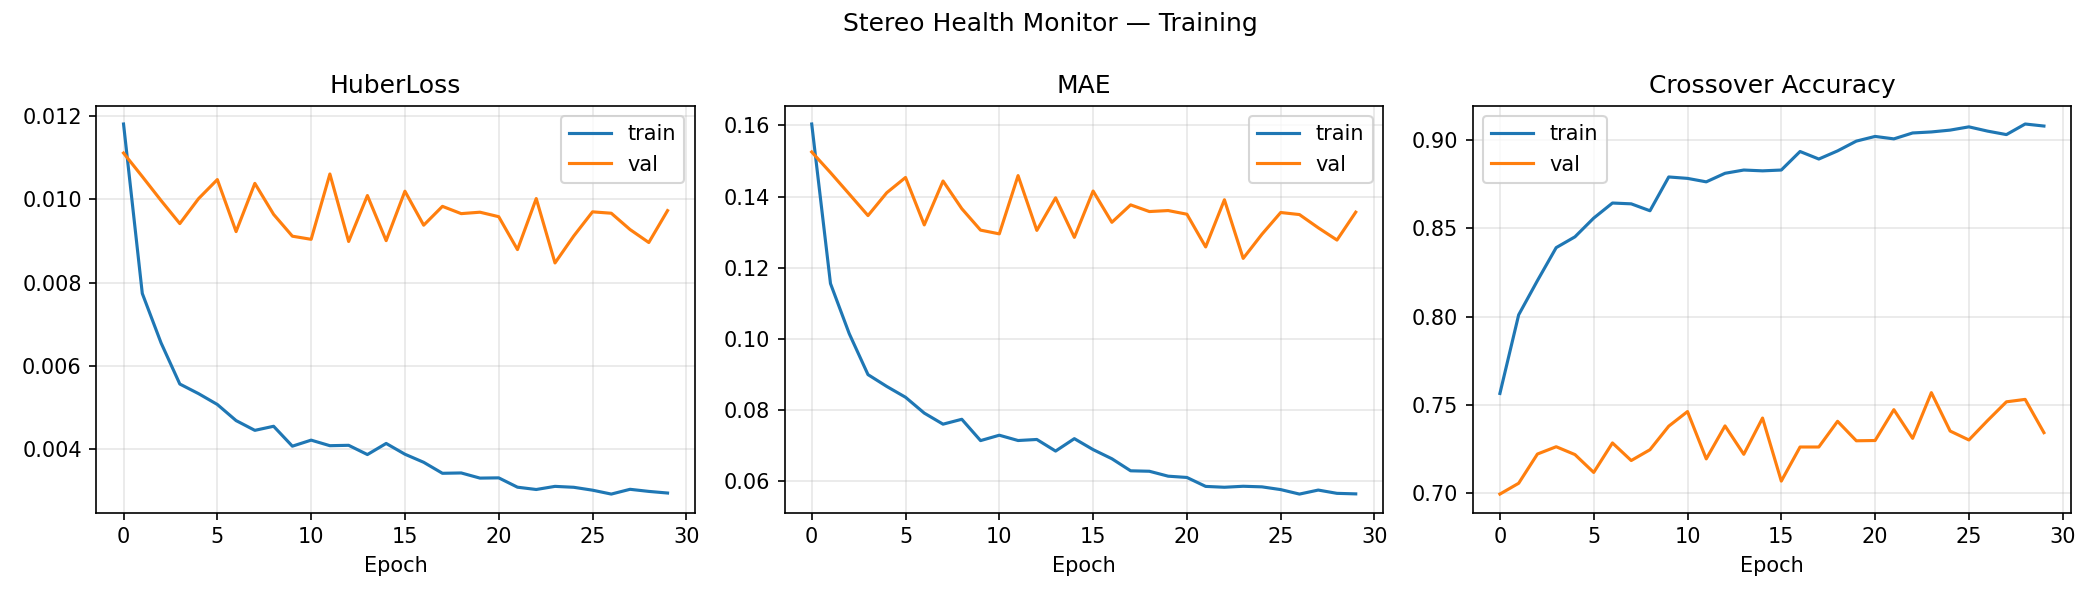
\includegraphics[width=\textwidth]{../health_monitor/training_curves.png}
    \caption{Training and validation curves over 30 epochs.
             Train MAE drops to 0.06; val MAE plateaus at $\approx$0.135,
             indicating moderate overfitting.}
\end{figure}

\begin{figure}[H]
    \centering
    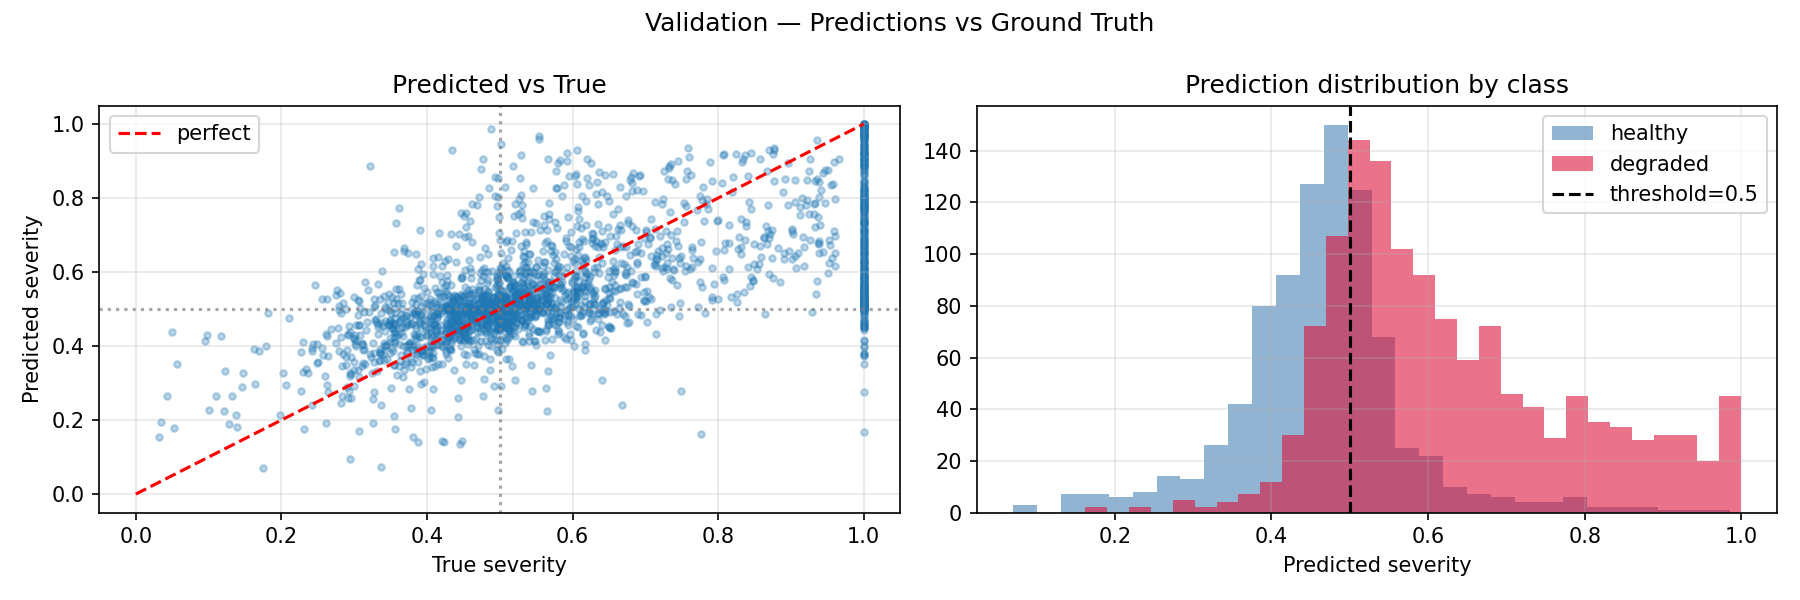
\includegraphics[width=\textwidth]{../health_monitor/val_predictions.png}
    \caption{Validation set predictions vs ground truth (left) and prediction
             distribution by class (right). Predictions now span the full $[0,1]$
             range — improvement over the previous version which was compressed
             to $[0.35, 0.75]$.}
\end{figure}

\begin{table}[H]
\centering
\begin{tabular}{lll}
\toprule
\textbf{Metric}          & \textbf{Value} & \textbf{Notes} \\
\midrule
Val MAE                  & 0.135          & Improvement from 0.158 \\
Val crossover accuracy   & $\sim$75\%     & Correct healthy/degraded classification \\
Sanity check crossover   & \textbf{90.5\%} & On held-out known conditions \\
Sanity check MAE         & 0.149          & On held-out known conditions \\
Prediction range         & Full $[0, 1]$  & Was compressed $[0.35, 0.75]$ before \\
\bottomrule
\end{tabular}
\caption{Summary of model performance metrics.}
\end{table}

% ---------------------------------------------------------------------------
\section{Model Sanity Check (Testing)}

To validate the model on known conditions, we sampled 3 windows each from
5 condition/traj combinations and ran the full model forward pass.
Each window shows 20 consecutive frames (left clean, right degraded)
with the predicted and ground-truth severity.

\subsection{Gaussian Blur — Mild (blur\_lv1, $\sigma = 0.5$)}

\begin{figure}[H]
    \centering
    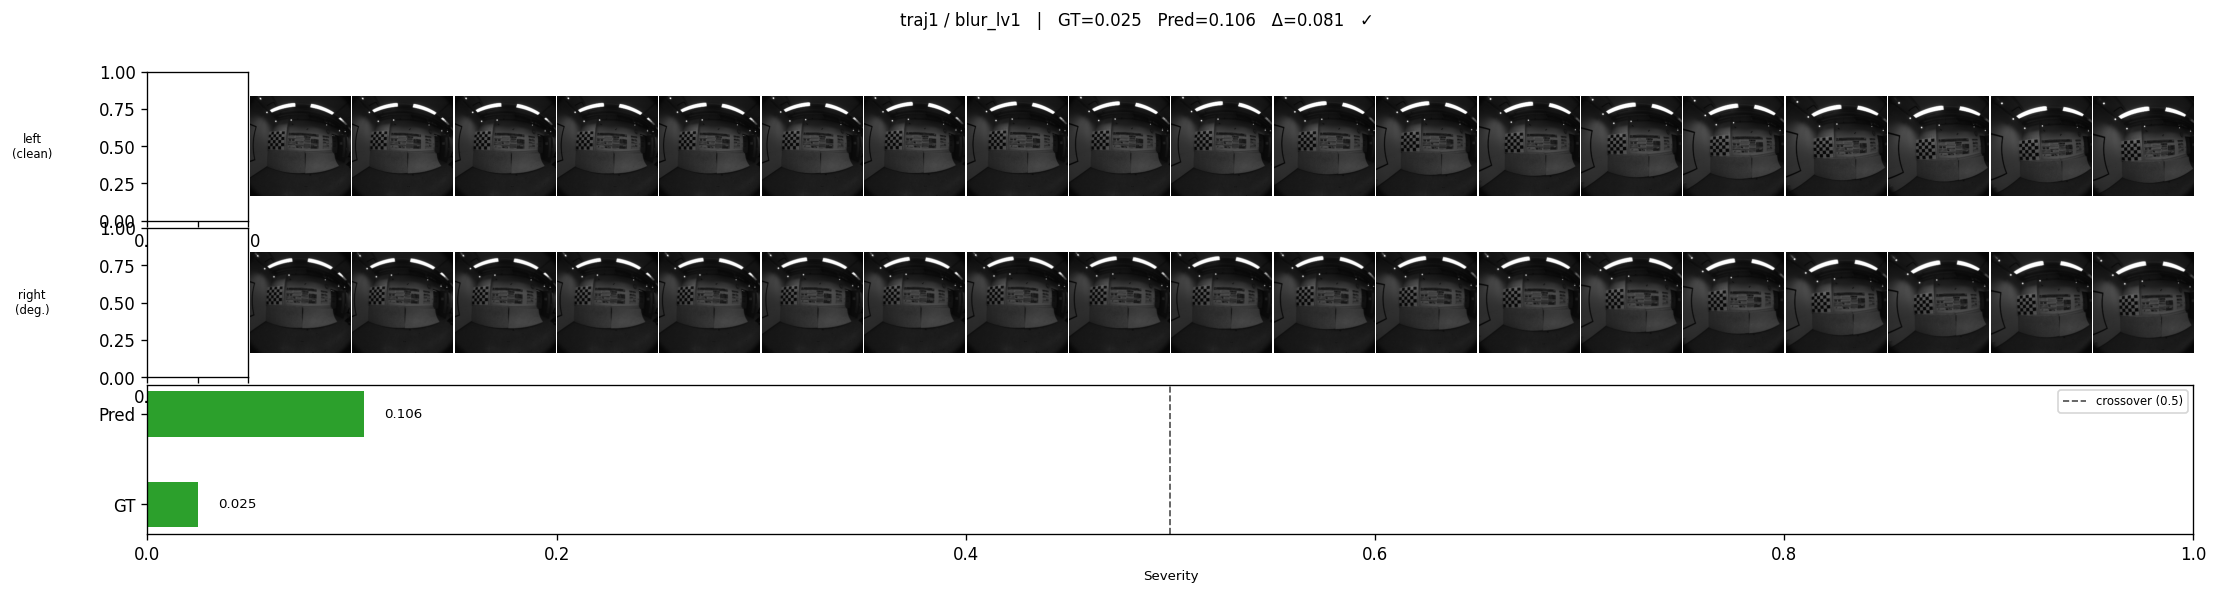
\includegraphics[width=\textwidth]{model_sanity_check_00_blur_lv1.png}
    \caption{Mild blur ($\sigma=0.5$). GT=0.025, Pred=0.106. The right image
             is barely distinguishable from the left. The model correctly
             predicts low severity ($<0.5$).}
\end{figure}

\subsection{Gaussian Blur — Severe (blur\_lv5c, $\sigma = 6.0$)}

\begin{figure}[H]
    \centering
    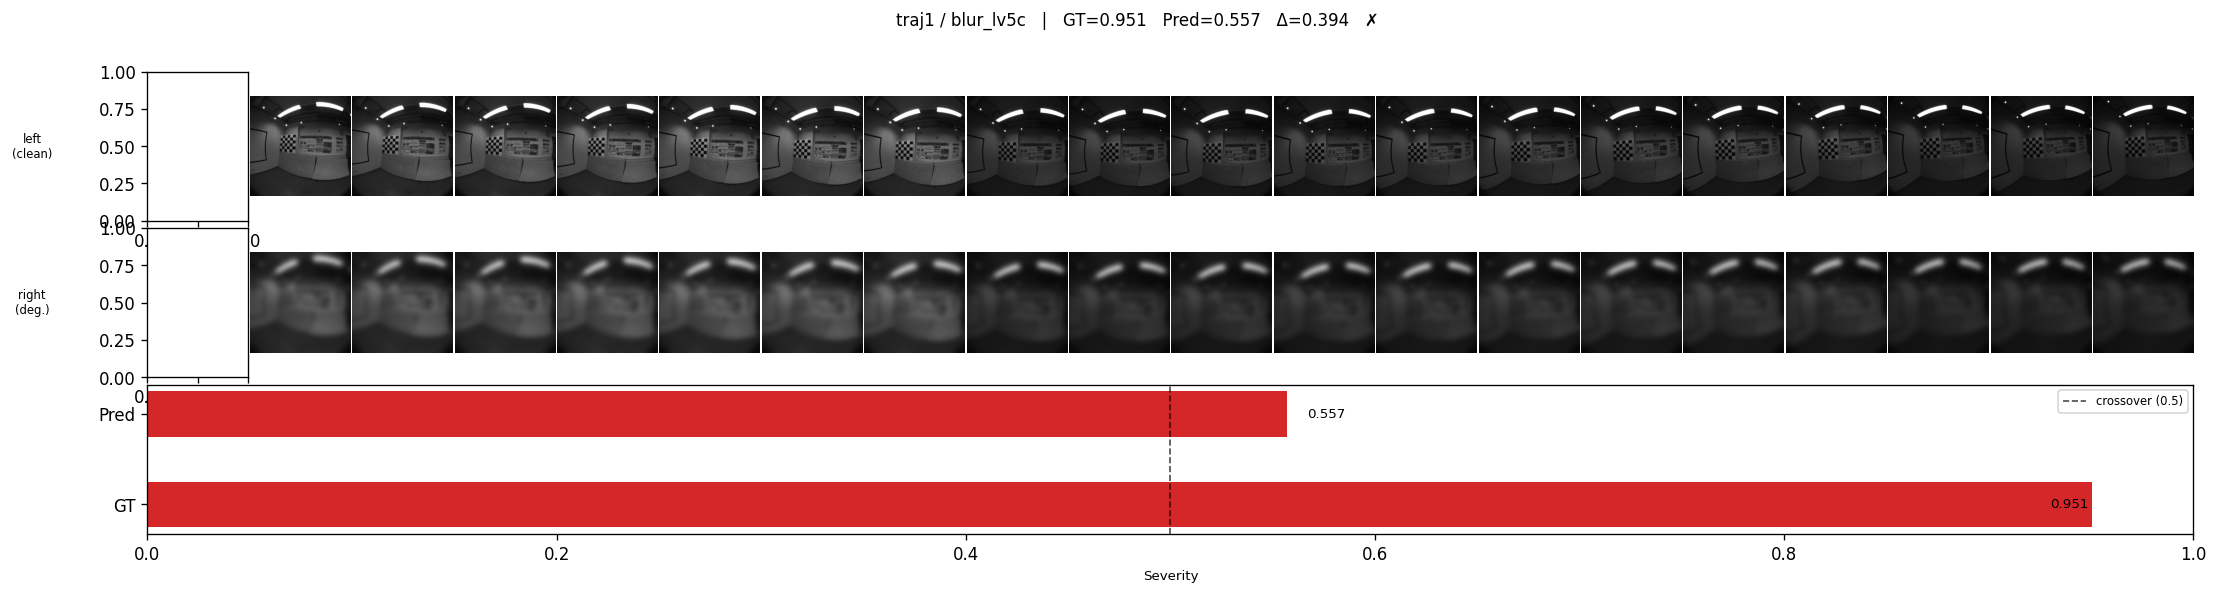
\includegraphics[width=\textwidth]{model_sanity_check_06_blur_lv5c.png}
    \caption{Severe blur ($\sigma=6.0$) — one step below the SLAM failure cliff.
             GT=0.951, Pred=0.557. The right image is heavily blurred.
             The model correctly crosses the 0.5 threshold but undershoots
             the true severity — the main remaining weakness.}
\end{figure}

\subsection{Motion Blur — Severe (mblur\_lv3b, length=25px)}

\begin{figure}[H]
    \centering
    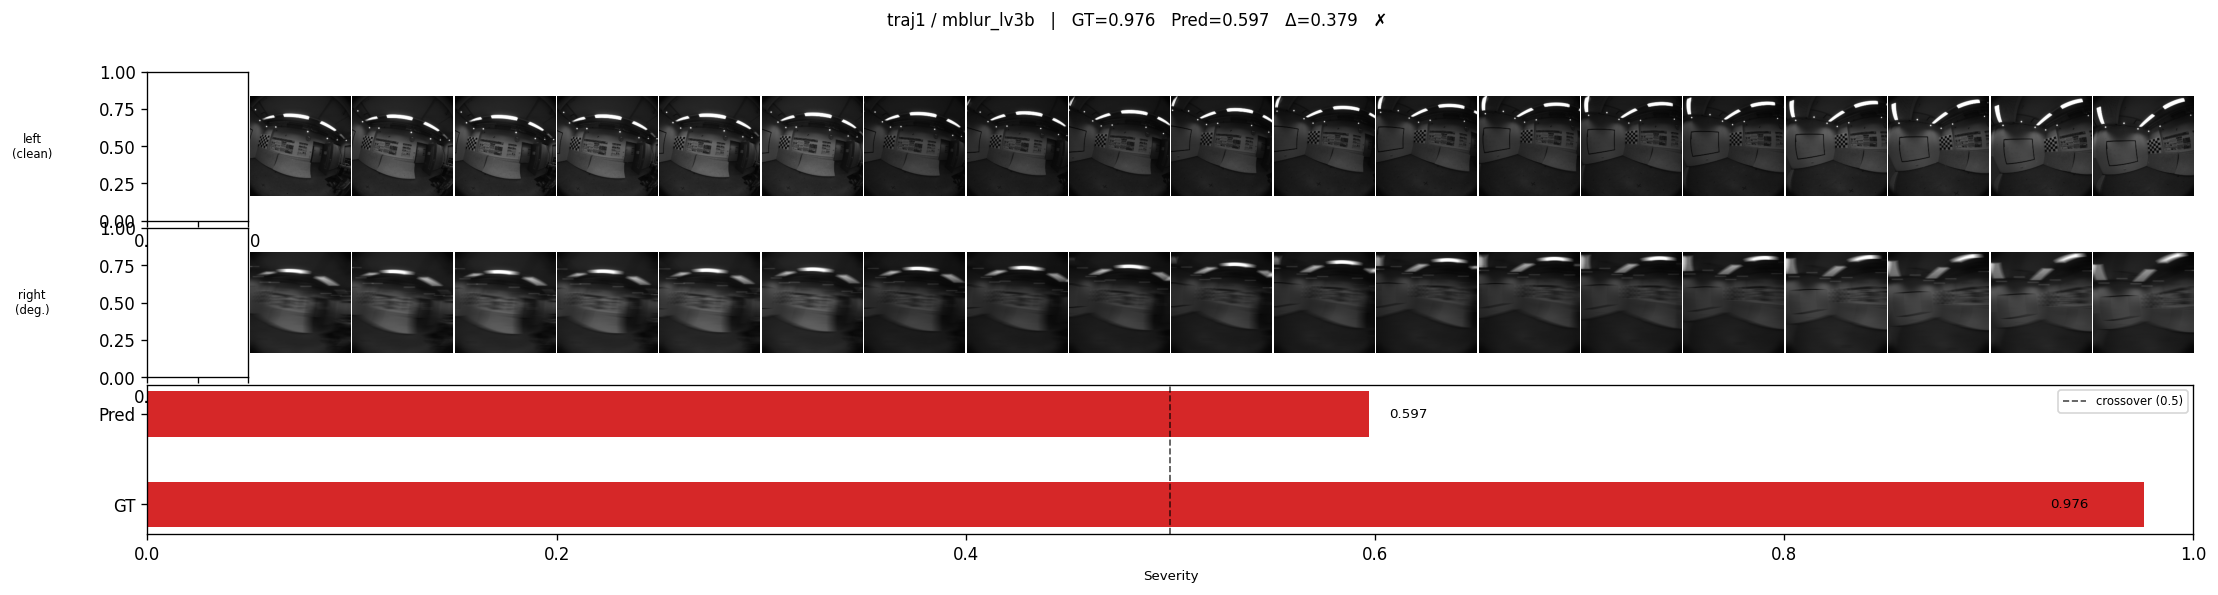
\includegraphics[width=\textwidth]{model_sanity_check_12_mblur_lv3b.png}
    \caption{Severe motion blur (length=25px, one step from SLAM failure).
             GT=0.976, Pred=0.597. The horizontal smearing is visible in the
             right image. Model correctly predicts degraded ($>0.5$) but
             undershoots the extreme severity.}
\end{figure}

% ---------------------------------------------------------------------------
\section{Key Findings}

\begin{enumerate}

    \item \textbf{The severity label is self-supervised and physically meaningful.}
          No manual annotation was needed. The mono-vs-stereo RTE ratio directly
          encodes when stereo stops being worth running.

    \item \textbf{The diff embedding is the right representation.}
          t-SNE analysis showed that $e_{\text{left}} - e_{\text{right}}$
          clusters clean pairs tightly near zero and pushes degraded pairs
          outward — giving the model a meaningful geometric signal to work with.

    \item \textbf{The model learns the correct direction of severity.}
          Mild blur $\to$ moderate blur $\to$ severe blur produces monotonically
          increasing predictions. The crossover at 0.5 is consistently respected.

    \item \textbf{The model correctly triggers the switch in 90.5\% of tested windows.}
          Crossover accuracy (healthy vs degraded classification) is the most
          operationally relevant metric --- and it is the strongest result.

    \item \textbf{Absolute severity values are underestimated at the extremes.}
          The model predicts 0.55--0.65 for conditions with GT severity $>0.9$.
          This is a calibration problem, not a structural one --- the model knows
          the condition is degraded, it just doesn't know \textit{how} degraded.

    \item \textbf{The train-val gap indicates overfitting.}
          Train MAE reaches 0.06 while val MAE plateaus at 0.135. Causes include
          limited trajectory diversity (2 sequences) and the weighted sampler
          aggressively upsampling rare healthy windows. Future work: more
          trajectories, label smoothing, or a softer sampling strategy.

\end{enumerate}

% ---------------------------------------------------------------------------
\section{Limitations and Future Work}

\begin{itemize}
    \item Only 2 trajectories used for training --- more scene diversity needed
    \item Backbone (layer4) partially unfrozen --- full fine-tuning may help
    \item Salt \& pepper and occlusion have cliff-only labels --- consider
          excluding them from training or treating as hard negatives
    \item Severity calibration at the extremes needs improvement ---
          temperature scaling or Platt scaling as post-processing
    \item Real-time inference not yet validated --- GRU hidden state could be
          maintained across frames for streaming operation
\end{itemize}

\end{document}
